\documentclass{article}
\usepackage[utf8]{inputenc}


\begin{document}

\begin{center}
\caption\textbf{HERRAMIENTAS DE BUSINESS ANALITYCS}
\end{center}
\\
\begin{itemize}
\item Análisis FODA:
\\Es una herramienta de análisis estratégico que nos permite analizar la situación interna y externa de una empresa o proyecto. Es como hacer una fotografía de la situación de nuestra empresa. Por eso, dado que esta situación no es estático, sino que evoluciona continuamente a lo largo del tiempo, además de utilizarlo para elaborar el plan de negocio de nuestra empresa, es bueno repetirlo posteriormente cada cierto tiempo. El objetivo es conocer la situación real en la que se encuentra la organización, empresa o proyecto en cada momento y, en función de ello, planear la estrategia de futuro más adecuada. El nombre de esta herramienta de análisis es un acrónimo de Fortalezas, Oportunidades, Debilidades y Amenazas. 
		\begin{center}
		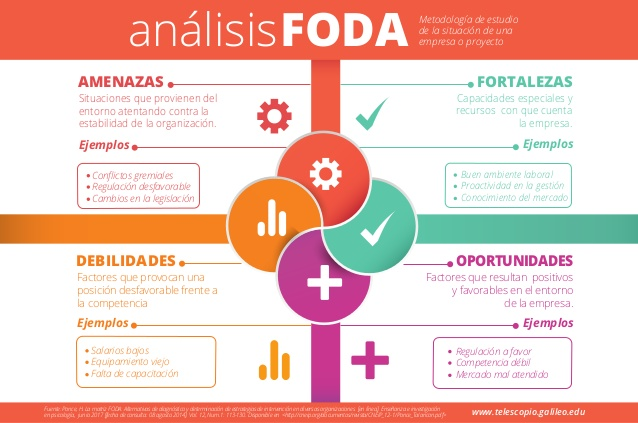
\includegraphics[width=15cm]{./Imagenes/Imagen3}
		\end{center}

	\end{itemize} 
	
	\begin{itemize}
\item Modelo de las 7 S:
\\A diferencia de la mayoría de las herramientas de análisis estratégico que suelen centrarse en el análisis externo, el Modelo de las 7 S, desarrollado a principios de los años 80 por Tom Peters y Robert Waterman, dos consultores de la firma McKinsey & Company, apunta directamente al interior de nuestra compañía. El modelo analiza, concretamente, 7 factores, cuyos nombres en inglés empiezan por S (de ahí el nombre de la herramienta, las 7 S) y que, según sus autores, son los 7 factores fundamentales de cualquier estructura organizativa:

- Estrategia (Strategy)\\
- Estructura (Structure)\\
- Sistemas (Systems)\\
- Estilo (Style)\\
- Valores compartidos (Shared values)\\
- Personal (Staff)\\
- Habilidades (Skills)
La idea del modelo es que las organizaciones no operan como un conjunto de silos estancos, sino más bien como una red de piezas interconectadas. Por eso es fundamental que los siete factores recogidos en el modelo estén alineados para que nuestra empresa tenga éxito. En este sentido, a la hora de implementar cualquier nueva estrategia, se deberá comprobar previamente todos ellos mantendrían su alineación, una vez implementada. Si la respuesta es que no para todos o parte de los factores, será necesario replantearse parte o la totalidad de la estrategia antes de proceder a su implementación. Para verlo más claro, lo mejor es dibujar un octógono y colocar cada una de las S en uno de sus vértices. Excepto los valores compartidos que, como son compartidos, los situaremos en el centro del octógono. Después, trazaremos líneas que vayan desde cada vértice hasta los demás.
		\begin{center}
		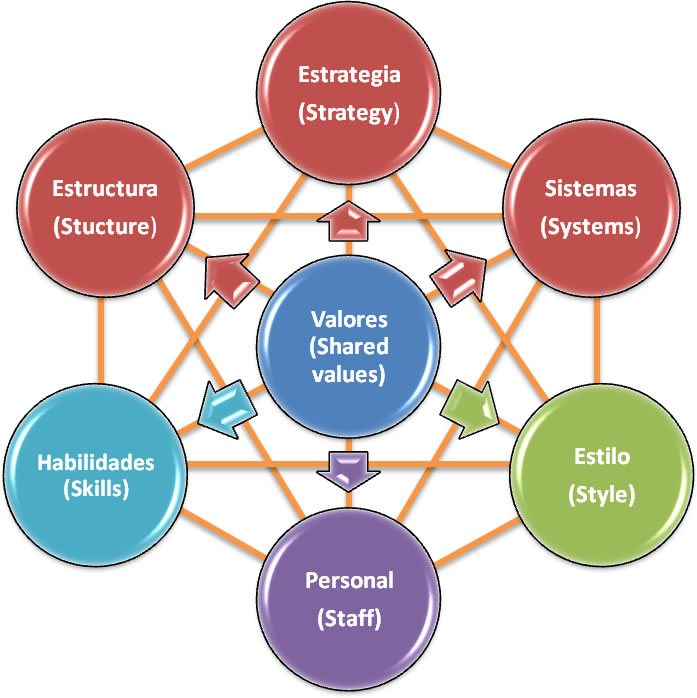
\includegraphics[width=15cm]{./Imagenes/Imagen4}
		\end{center}
	\end{itemize} 

\end{document}
